\stepcounter{chapter} % This line will increment the chapter counter
\chapter*{Clustering} % This line will create an unnumbered chapter
\addcontentsline{toc}{chapter}{\protect\numberline{\thechapter}Clustering} % This line will add the chapter to your table of contents
\markboth{Clustering}{} % This line will set the header
\vspace{-10mm}
Before starting the cluster analysis, we selected the variables in the dataset, dropping nominal ones, i.e., \texttt{name}, \text{album\_name}, \text{artists} and categorical/discrete ones (like \texttt{key} and \texttt{genre}). We decided to also drop the \texttt{processing} column because, observing the number of unique values and the distribution, is likely to be discrete (like key and time signature); moreover we don't have an accurate description of the variable, so it would be difficult to give an interpretation to its possible contribution in a cluster (although from the PCA there was a glimpse of a contribution in relation to key). The remaining features are 12: ['duration\_min', 'popularity', 'danceability', 'energy', 'loudness', 'speechiness', 'acousticness', 'instrumentalness', 'liveness', 'valence', 'tempo', 'n\_bars'].\\
The clustering techniques were applied to two datasets: one with 15000 records and 12 features, and another with 10575 records and 12 features, excluding outliers (rejected based on the criteria described in Data Understanding, IQR and Standard Deviation, see \ref{outliers_detection}); the cutoff this time is smaller (about 29\% of the samples) because we dropped some columns that contained the outliers that were cut in the first case. Henceforth we will call $\mathbf{F}$ the full dataset with all samples and $\mathbf{C}$ the cut dataset without outliers. The best performing dataset was chosen for each algorithm. The process involved three steps: using all features, using only selected features, and evaluating performance. The selected features were determined by a selection algorithm based on feature importance for cluster separation (see Fig. \ref{fig:parallel}).
\section{Centroid-based clustering}
\subsection{Choice of $k$}
We applied the following techniques for choosing the optimal value of $k$, both methods provide heuristic approaches to determine the number of clusters.
\begin{figure}[ht]
\begin{minipage}{.6\textwidth}
\textsc{Elbow Method}: involves running the k-means algorithm for a choosen range of values of $k$. For each value of $k$, the Sum of Squared Errors (SSE) is calculated and stored in a list. The SSE tends to decrease toward 0 as we increase $k$ (i.e., as the number of clusters increases, the distance from each data point to its closest centroid gets smaller). The “elbow” in the plot of SSE versus $k$ is considered as an indicator of the appropriate number of clusters. This “elbow” is the point representing the value of $k$ beyond which the decrease of SSE is no longer evident. When the elbow point is not distinguishable, we can use \texttt{KneeLocator} from the library \texttt{kneed}.
\end{minipage}
\begin{minipage}{.4\textwidth}
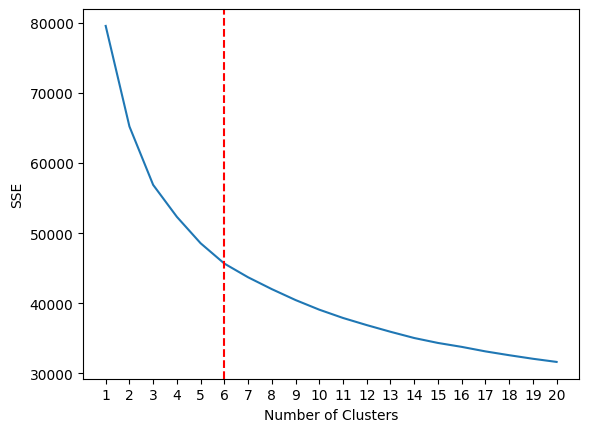
\includegraphics[width=\textwidth]{img/sse_all.png}
\end{minipage}
\end{figure}
\begin{figure}[ht]
\begin{minipage}{.6\textwidth}
\textsc{Silhouette Method}: measures (range -1 to 1) how similar an object is to its own cluster compared to other clusters; a high value indicates that the object is well matched to its own cluster and poorly matched to neighboring clusters. If most objects have a high value, then the clustering configuration is appropriate. In this analysis the silhouette is calculated using a precomputed euclidean distance matrix (we used \texttt{pdist}, \texttt{squareform} from \texttt{scipy.spatial.distance}).
\end{minipage}
\begin{minipage}{.4\textwidth}
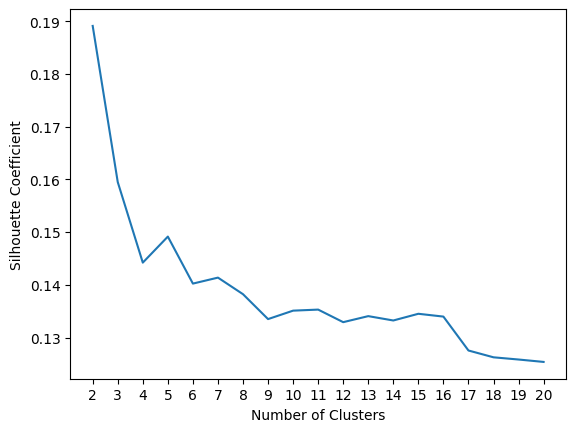
\includegraphics[width=\textwidth]{img/sil_all.png}
\end{minipage}
\end{figure}
\newpage
\subsection{Evaluation techniques}
Clustering evaluation is first performed by calculating \textbf{SSE} and \textbf{silhouette score}, for both datasets. For further validation we implemented a code that provides a thorough evaluation of the KMeans clustering results, taking into account the possibility of obtaining similar results by chance:
\begin{enumerate}
\item \textbf{Compute Correlation:} correlation (using the Pearson correlation coefficient) between the distance matrix of the data and the ideal similarity matrix, that is a binary matrix where 1 indicates that two points belong to the same cluster and 0 otherwise. 
\item \textbf{KMeans Evaluation:} we then evaluate the significance of the clustering result by comparing it with the results of clustering on randomized datasets. This is done by: randomizing the data, computing the KMeans clustering for the randomized data, computing SSE and correlation for the randomized data, storing the results and repeating the steps for a choosen number of permutations ($200$ for SSE evaluation, $100$ for Silhouette).
\item \textbf{Plots:} histogram and Kernel Density Estimation (KDE) plot of SSE and correlations for the randomized datasets. The original values of SSE and correlation are represented by a dashed vertical line. 
\end{enumerate}
If the original SSE is significantly lower than the permuted ones, it suggests that the clusters found by K-means are meaningful and not a result of random chance. On the other hand, if the original SSE is not much lower than the permuted ones, it suggests that the K-means solution might not be capturing any meaningful structure in the data. Then, if the original correlation is significantly different from the mean value given by permutations, it suggests that the clusters found by K-means are meaningful and not a result of random chance.

\subsection{K-Means}
Based on the assumptions above, for all the $12$ features the results are: $k=4$ for $\mathbf{F}$-dataset and $k=5$ for $\mathbf{C}$-dataset. The one that performed slightly better (but still poor, sil$=0.21$) is $\mathbf{F}$, with the following parallel chart:
\begin{figure}[H]
    \centering
    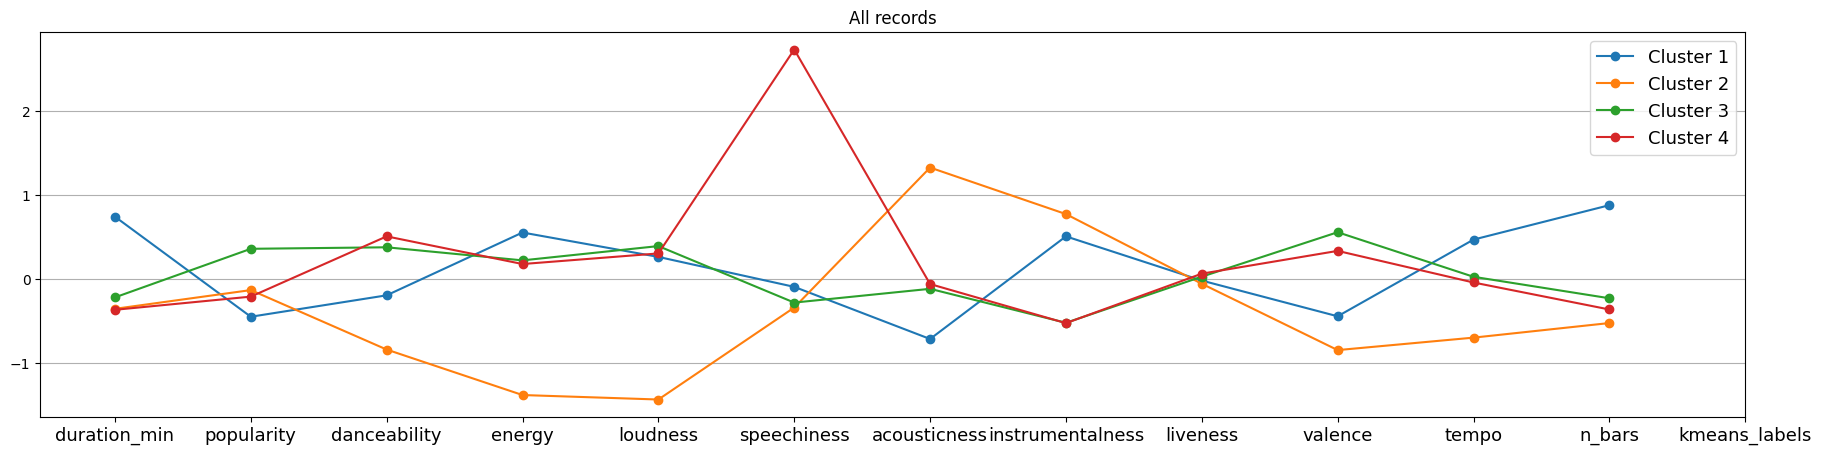
\includegraphics[scale=0.35]{img/parallel_all_kmeans.png}
    \caption{Parallel Line Chart; full dataset with all features. Points represents centroids with respect to the features.}
    \label{fig:parallel}
\end{figure}
\begin{wrapfigure}{r}{0.35\textwidth}
\vspace{-1cm}
\caption{2D and 3D plots: full dataset with selected features.}
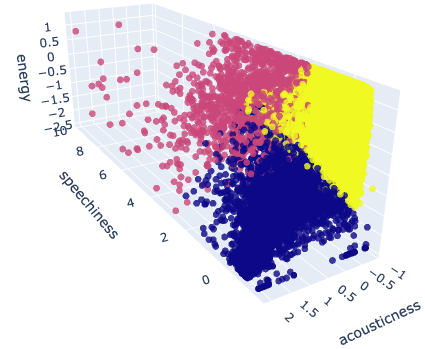
\includegraphics[width=\linewidth]{img/3d_kmeans.png}
\vspace{2cm}
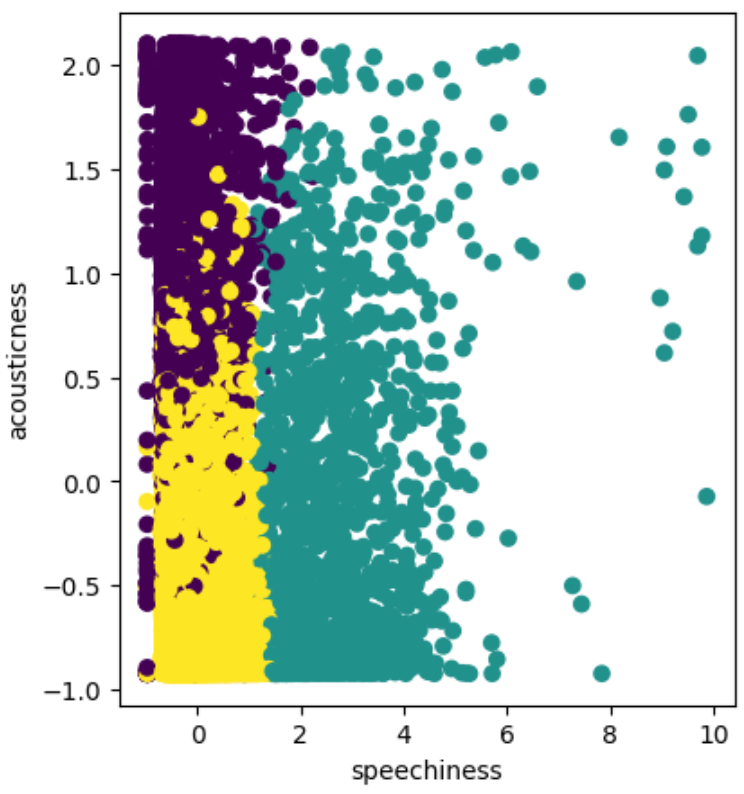
\includegraphics[width=0.7\linewidth]{img/2d_kmeans.png}
\vspace{-5cm}
\end{wrapfigure}
We decided to try to select only those features that generate more pronounced separation between centroids (either based on the parallel chart display or by calculating them with an appropriate algorithm). For the two datasets they were found to be more "important":
\begin{verbatim}
F -> ['speechiness', 'acousticness', 'energy']
C -> ['instrumentalness', 'acousticness', 'energy']
\end{verbatim}
Combinations with the 6, 5, or 4 most important features have been tested, but the results are poor. So we repeat the analysis using only the 3 most important features for each dataset. From the study of the SSE and silhouette score we obtain $k_\mathbf{F}=3$ and $k_\mathbf{C}=4$. \\
After fitting the two kmeans, the best silhouette score is $0.51$ ($\mathbf{F}$-dataset). As specified above, for further validation, correlations and SSE are calculated through permutations of the same data.
\begin{figure}[H]
\vspace{0.5cm}
    \centering
    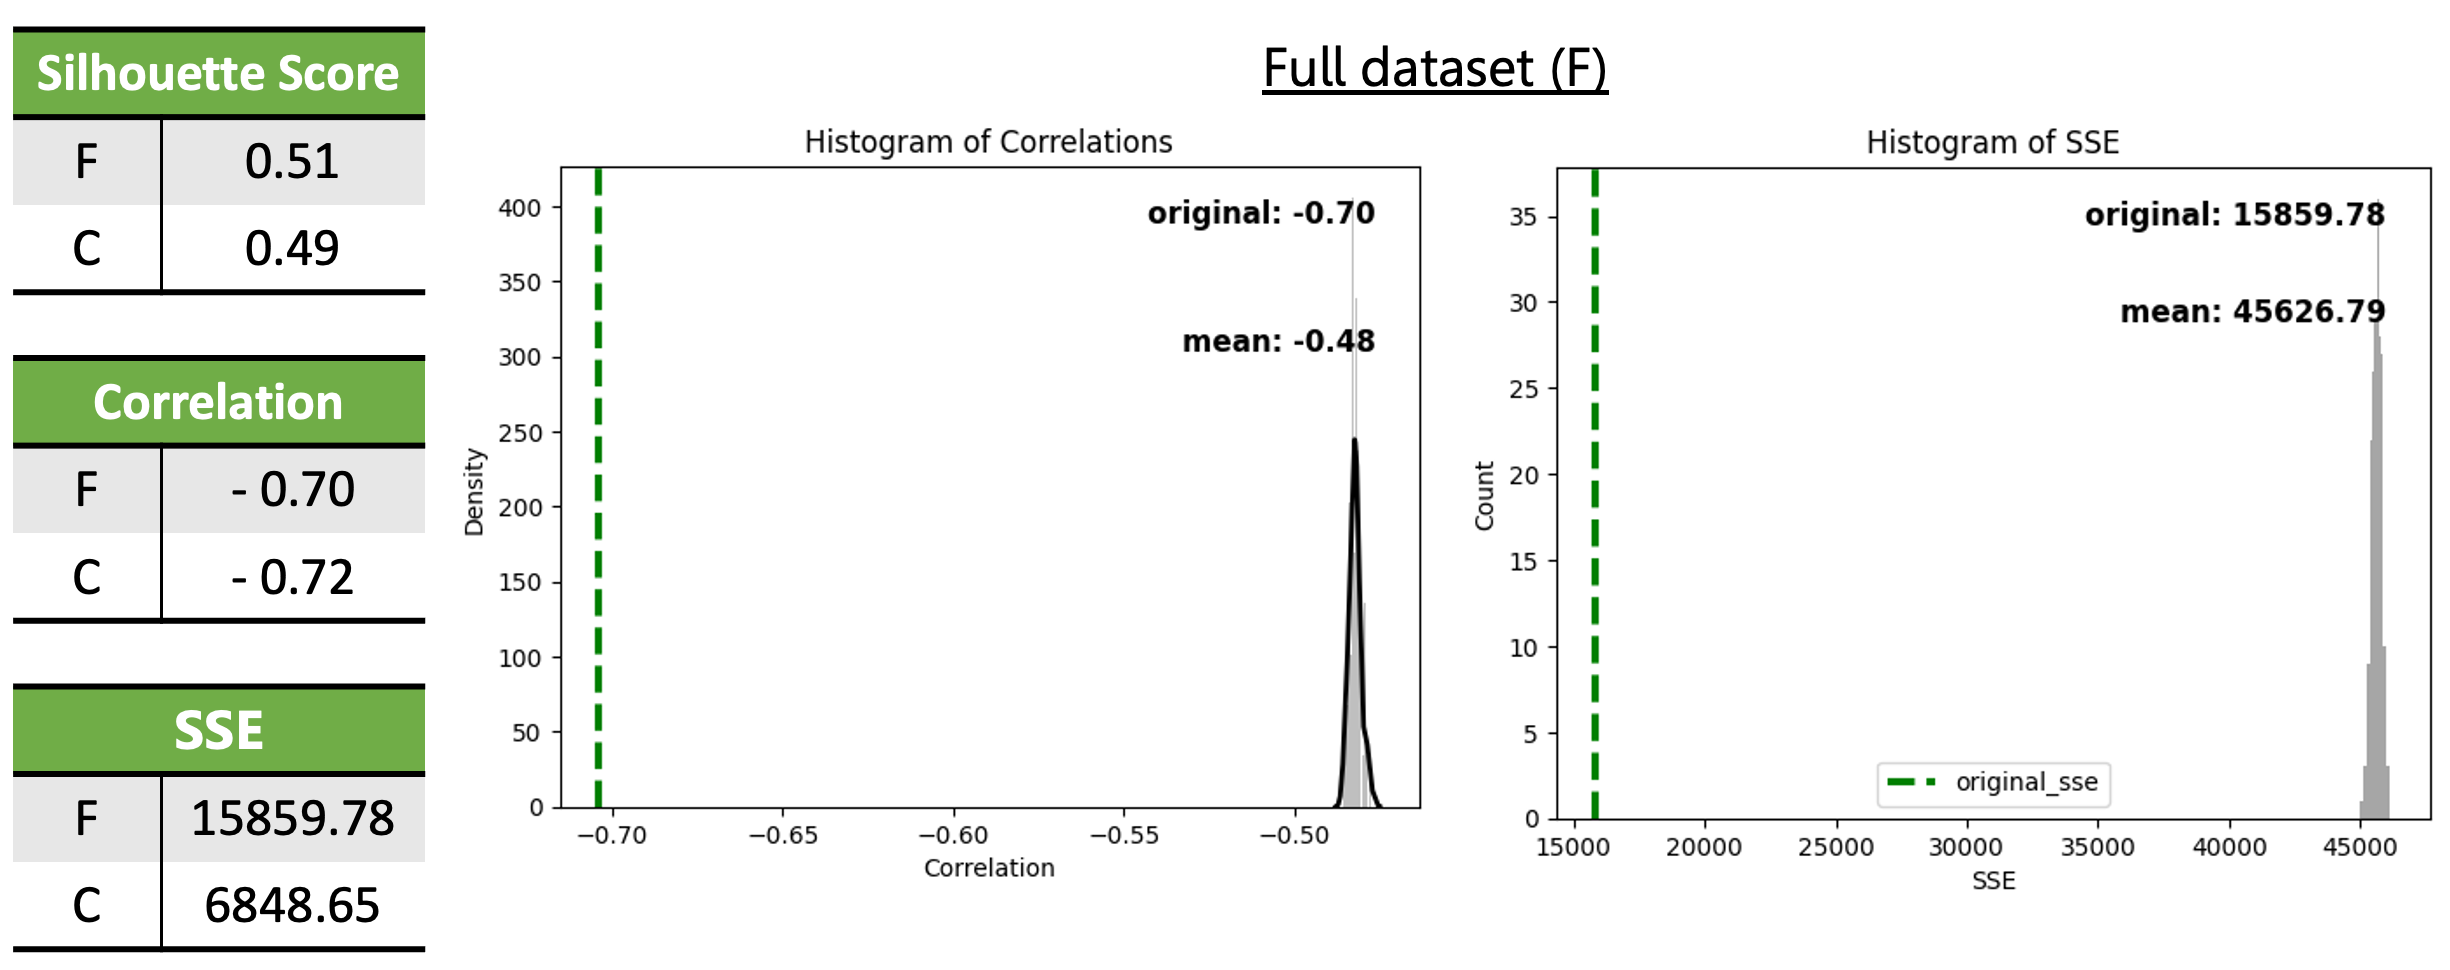
\includegraphics[scale=0.35]{img/final_kmeans.png}
    \caption{Results of KMeans evaluation, the histogram plot refers to the full dataset. F: full dataset, C: dataset without outliers.}
    \label{fig:enter-label}
\end{figure}
Both datasets show a negative correlation because it's calculated between the distance matrix and the ideal similarity matrix. We can try to give an interpretation to the clusters generated by the analysis:\\
\begin{wrapfigure}{l}{0.4\textwidth}
\vspace{-0.8cm}
    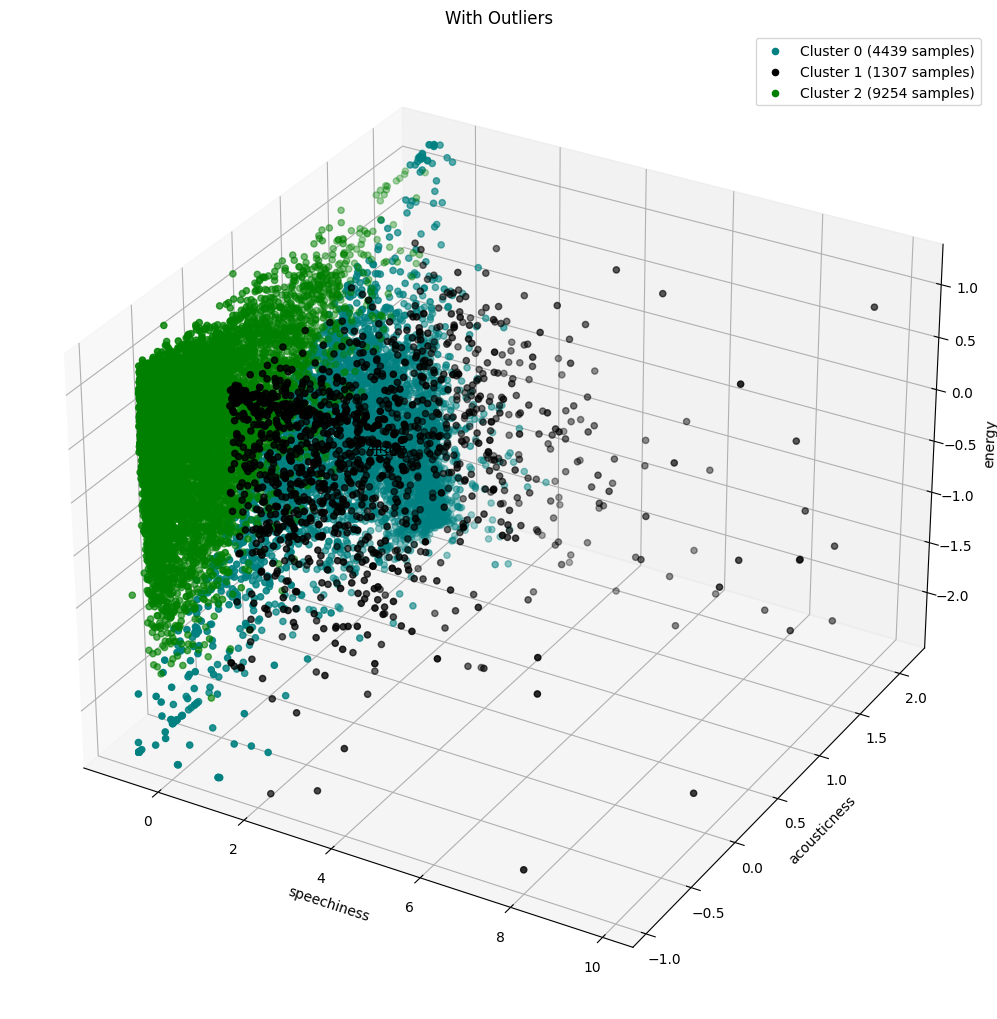
\includegraphics[width=\linewidth]{img/kmeans_FINALE.png}
\caption{Teal: Cluster 0, Black: Cluster 1, Green: Cluster 2}
\vspace{-2cm}
\end{wrapfigure}
\begin{itemize}
    \item Cluster \texttt{0}: \textbf{4439} samples; tracks with low energy and speechiness and high acousticness, it could contain mainly instrumental low-energy acoustic songs.
    \item Cluster \texttt{1}: \textbf{1307} samples; tracks with ascending speechiness, high energy and low acousticness, maybe containing rap songs.
    \item Cluster \texttt{2}: \textbf{9254} samples; tracks with low speechiness and acousticness and high energy, it may contain dance music.
\end{itemize}
\subsection{Bisecting K-Means}
Bisecting k-means is a hybrid approach between Hierarchical Clustering and K-means Clustering. Instead of partitioning the data set into $k$ clusters in each iteration, bisecting k-means algorithm splits one cluster into two sub clusters at each bisecting step (by using k-means) until $k$ clusters are obtained.\\
\begin{wrapfigure}{l}{0.6\textwidth}
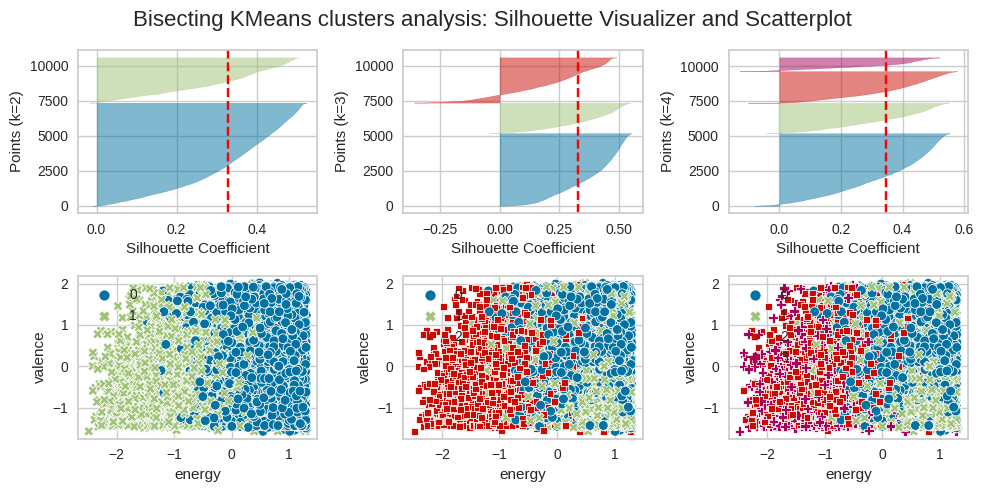
\includegraphics[width=\linewidth]{img/bkmeans_ev2.png}
\caption{Silhouette Visualizer, from $k=2$ to $k=4$.}
\label{bk_viz}
\end{wrapfigure}
In this section we performed the analysis with $k_\mathbf{F}=3$ and $k_\mathbf{C}=4$ and a varying number of features, from 12 down to 3 (based on importance), computing SSE and Silhouette Coefficient for each set of features. From the results, it appears that the $\mathbf{C}$ dataset (without outliers) performs better (but still gives bad performances) in terms of both SSE ($53130.08$) and Silhouette ($0.26$) for $4$ features: ['acousticness', 'energy', 'loudness', 'valence'] for $\mathbf{F}$ and ['instrumentalness', 'acousticness', 'energy', 'valence'] for $\mathbf{C}$. Although the results are bad (SSE greater than 50000), to attempt further visualization we used Silhouette Visualizer from the yellowbrick library, which generates a series of silhouette plots and scatterplots for a variable number of clusters (in this case 2 to 4, Fig. \ref{bk_viz}).
\section{Density-based clustering}
Density-based clustering algorithms like DBSCAN can identify clusters of arbitrary shapes in datasets. This is an advantage over other clustering algorithms that assume clusters are spherical or have other predefined shapes. Additionally, DBSCAN can handle noise and outliers in the data, and does not require the number of clusters to be specified in advance.
\subsection{DBSCAN}
Again we run the algorithms on both the full dataset ($\mathbf{F}$) and the dataset without outliers ($\mathbf{C}$) to compare performance, both scaled with StandardScaler. Both datasets are tested with all features and then with the previously chosen features for kmeans analysis. The other feature selections did not affect the final results much, so we assumed that using the same attributes might have led to a better comparison between the two algorithms.\\
In order to choose the best parameters, we determined the optimal value of epsilon (eps), by plotting the $k$-th nearest neighbor distances for each data point in a given dataset, and then using the “elbow method” to find the optimal eps value (using again \texttt{KneeLocator} from \texttt{kneed}).
\begin{figure}[H]
    \centering
    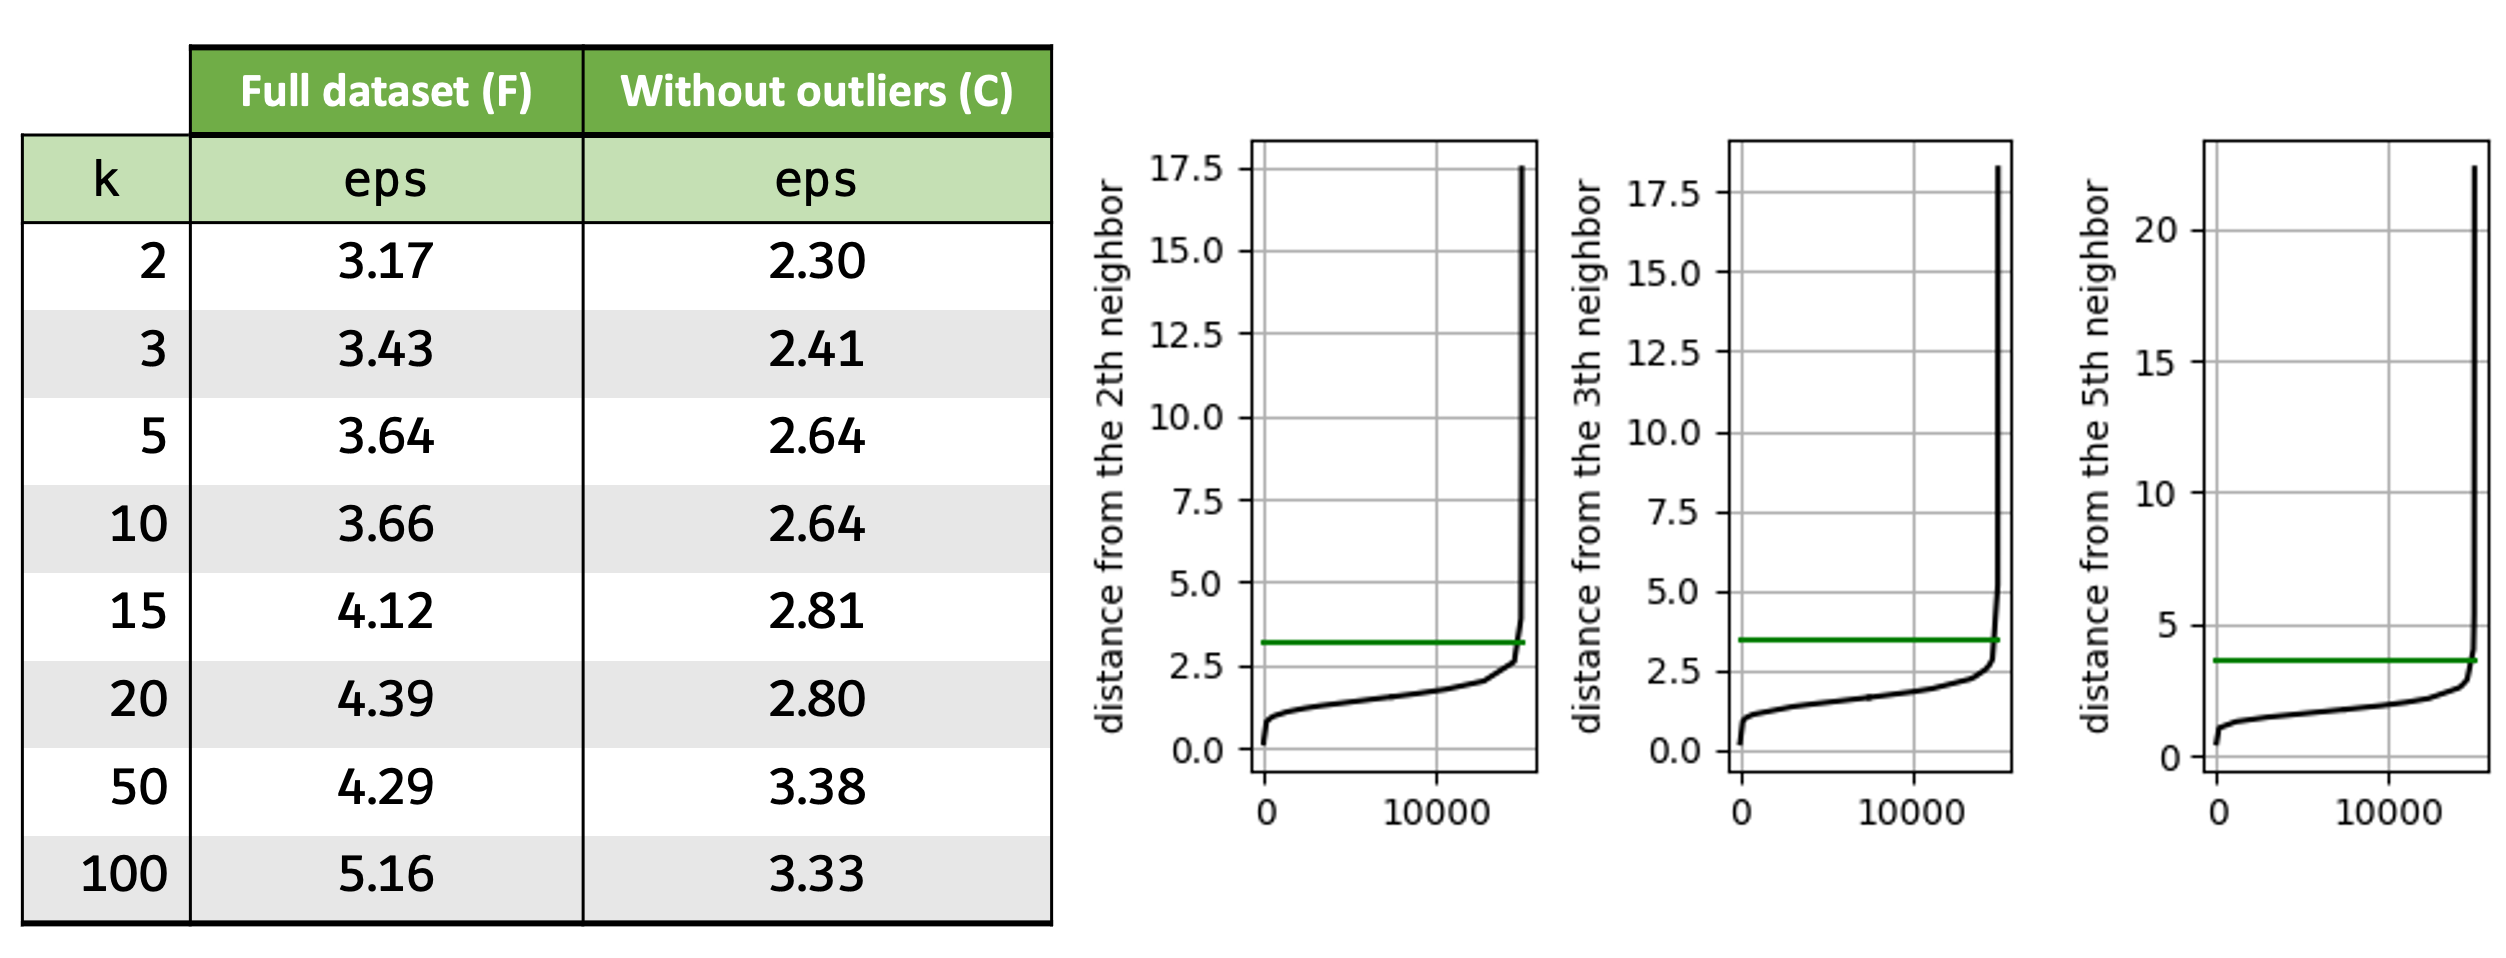
\includegraphics[scale=0.3]{img/eps_dbscan.png}
    \caption{Values of $k$ and \texttt{eps} for the datasets with all features.}
    \label{fig:enter-label}
\end{figure}
\begin{wrapfigure}{l}{0.4\textwidth}
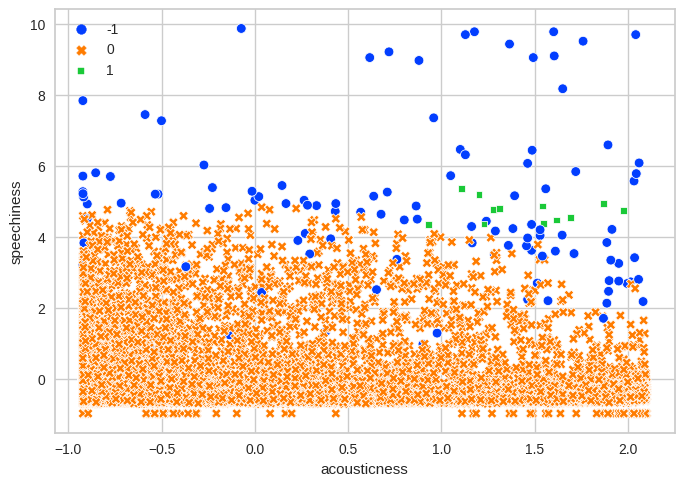
\includegraphics[width=\linewidth]{img/dbscan.png}
\caption{DBSCAN: Full Dataset, eps=0.75, minPts=12, sil\_score=0.59}
\vspace{-1cm}
\label{fig:dbscan}
\end{wrapfigure}
Because of the poor results with these configurations, we tried choosing a single eps value (average value of the two lists of values seen before, so $3.72$ for $\mathbf{F}$ and $2.10$ for $\mathbf{C}$) testing a wider range of k ($2$ to $51$) to find the winning combination. The best results are: \texttt{Full Dataset, eps=3.72, minPts=2, silhouette=0.45}.\\
Then we tried the same procedure by selecting, for each dataset, the same features selected for the kMeans (so we could make a better comparison); the results are: \texttt{Full Dataset, eps=0.75, minPts=12, silhouette=0.59}.\\
Despite having a convincing silhouette value, we discovered that the clustering is really very unbalanced (Fig. \ref{fig:dbscan}), since almost all the points are in the first cluster (orange), very few points are in the second cluster (green) and the others are all noise points (blue).
\section{Hierarchical clustering}
We decided to perform hierarchical clustering with Euclidean and Manhattan distances (precomputed) as metrics, and \texttt{single}, \texttt{complete}, \texttt{ward} and \texttt{average} linkages. By setting \texttt{n\_clusters}$=3$ (in order to compare results with KMeans analyisis), we used an algorithm that tested different combinations of distance-linkage returning a silhouette score. Also for the hierarchical clustering analysis, we tested the procedure first on the datasets with all features and then selecting the same features used for the second part of the KMeans. The best results were given by the configuration: dataset $\mathbf{F}$, \texttt{euclidean} distance, \texttt{single} linkage, $\texttt{sil\_score}=0.93$. The high value of silhouette score is unfortunately due to the large imbalance of the clusters: in fact, it is noticeable that there is a cluster that contains almost all the points in the dataset and then smaller clusters formed by single points. So we tried to see if the other linkages, although with lower silhouettes, could generate better separation.
\begin{figure}[H]
    \centering
    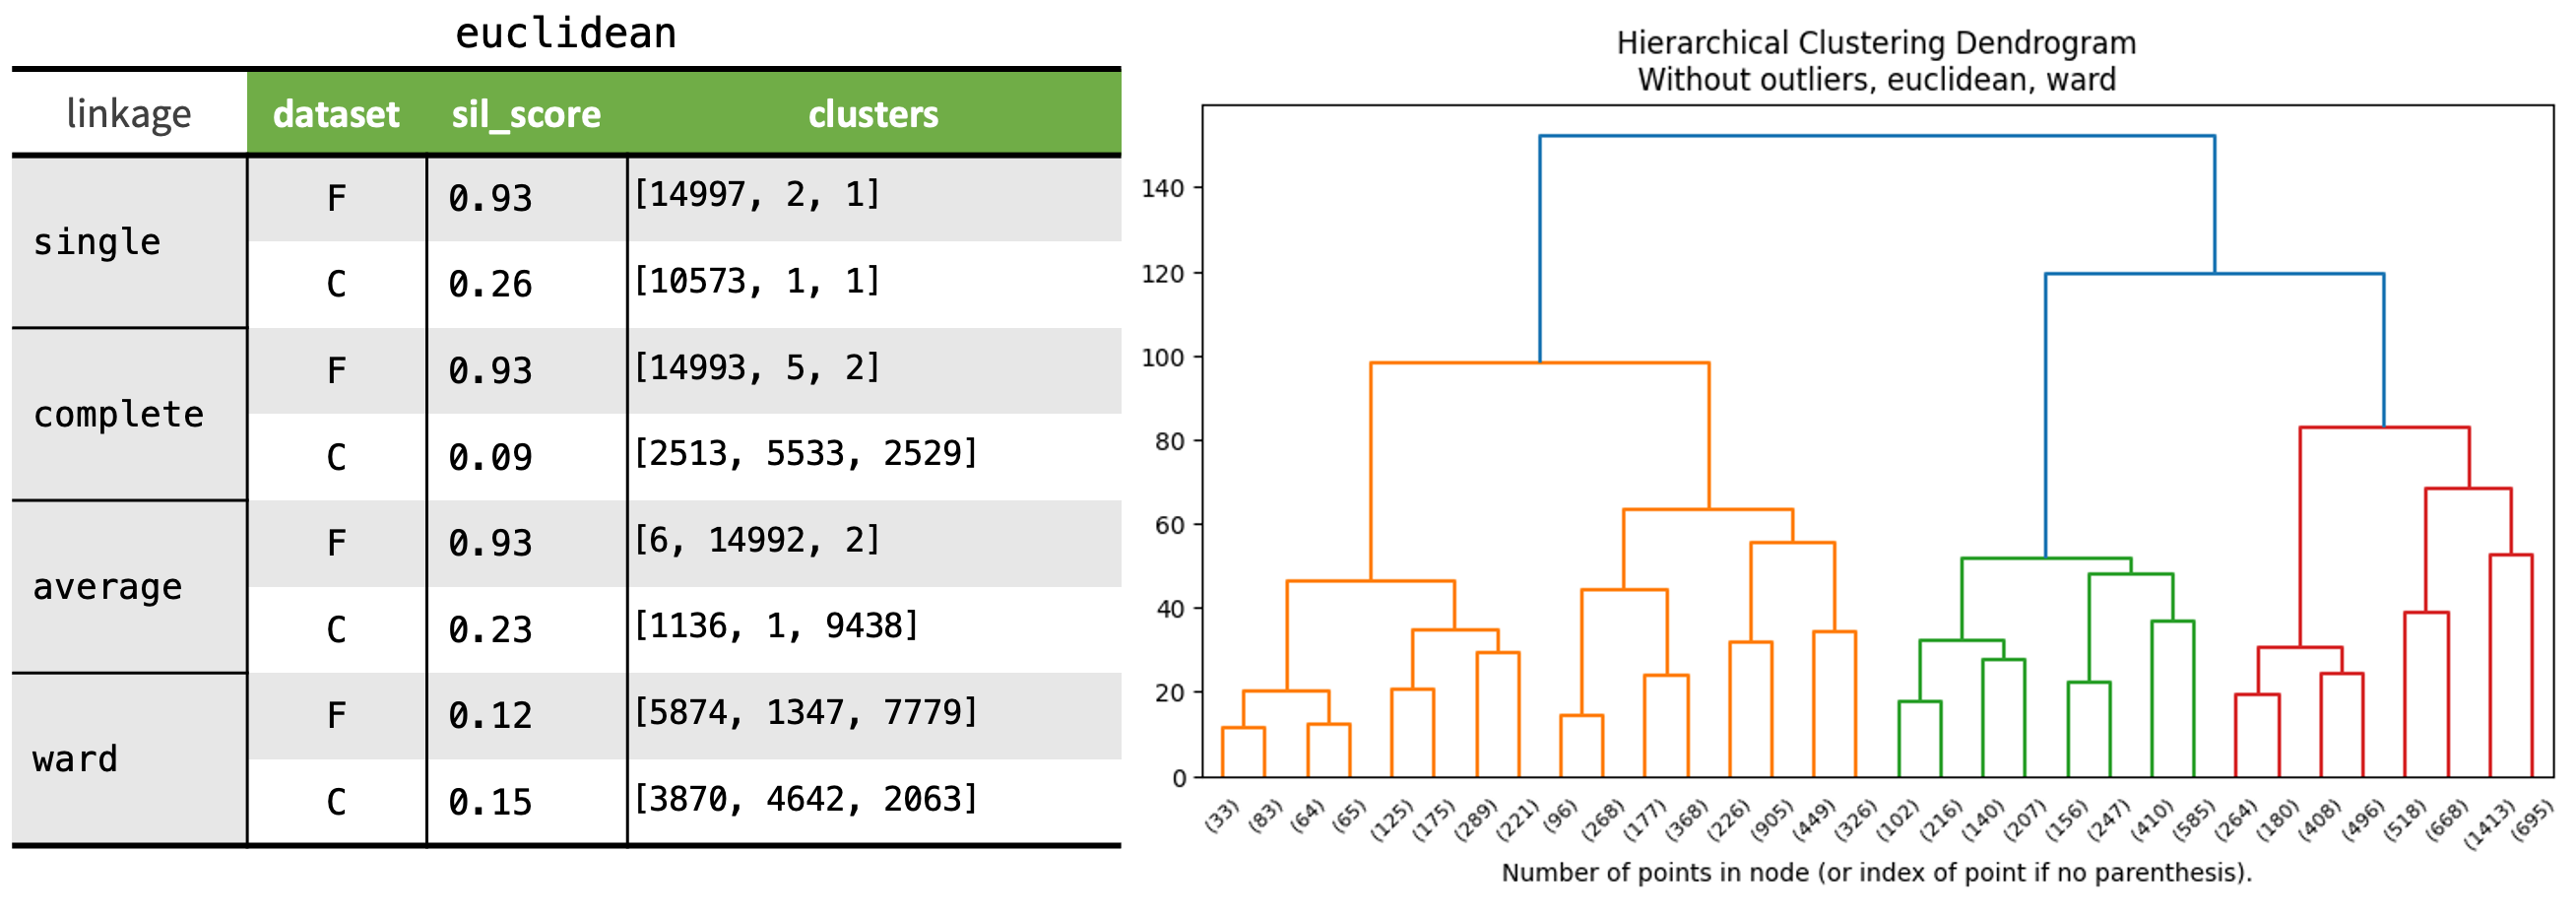
\includegraphics[scale=0.35]{img/hier_final2.png}
    \caption{Silhouette Scores of different combinations of dataset/linkage using euclidean distance.}
    \label{fig:enter-label}
\end{figure}
\noindent The C-euclidean-ward combination creates more balanced datasets, at the expense of a very low silhouette value.
\section{Final discussion}
Having reached this point, we can conclude that: DBSCAN is unable to provide optimal clustering, despite having tested several choices of eps and minPts, because it results mainly in large clusters that include almost the entire dataset, then only noise points; even the hierarchical methods produce highly unbalanced clusters. \\
\textbf{K-Means}, applied to a dataset with \textbf{selected features}, proved to be the only algorithm capable of separating some clusters in a balanced way with an acceptable silhouette value.